\documentclass{article}
\usepackage{graphicx}
\usepackage{amsmath}
\usepackage{enumitem}
\usepackage{float}
\usepackage{listings}
\usepackage{xcolor}
\usepackage[a4paper, margin=1in]{geometry}

% Custom information
\newcommand{\className}{Course: Automatic Control Systems – ASEN 5114-001 – Spring 2025}
\newcommand{\professorName}{Professor: Dale Lawrence}
\newcommand{\taName}{Teaching Assistant: Anantha Dhruva}
\title{Homework 1 \\ \className \\ \professorName \\ \taName}
\author{Steve Gillet}
\date{\today}

\lstdefinestyle{matlabstyle}{
    language=Matlab,              % Specify the language
    basicstyle=\ttfamily\footnotesize\color{black}, % Code font
    keywordstyle=\color{blue}\bfseries, % Keywords in blue
    stringstyle=\color{green},    % Strings in green
    commentstyle=\color{magenta}, % Comments in magenta
    numbers=left,                 % Line numbers on the left
    numberstyle=\tiny\color{black},% Line number style
    stepnumber=1,                 % Line number increment
    breaklines=true,              % Line breaking
    frame=single,                 % Border around code
    backgroundcolor=\color{white},
    tabsize=4,                    % Tab size
    showstringspaces=false,       % Don't show spaces in strings
}

\begin{document}

\maketitle
\textit{
    "Due: Monday, February 3, 2025 at 11:59 pm on Canvas. Please assemble a single PDF file for
    submission that includes your Matlab/Simulink code/diagrams, plots, and explanations of your
    work and the results. Label sections to correspond with those in the assignment. Don’t make it
    difficult to locate the text/code/plots for each section."
}

\section*{1.}

\textit{
    "[10pts] Find the parameters $R_M$, $L_M$, $K_\tau$, $J_M$, and $K_B$ from the motor specification sheet, noting
    units. Also, find the total gear ratio N from the motor shaft to the load shaft, and estimate the
    load shaft moment of inertia $J_L$. Use these to quantify the parameters in the transfer function
    relating $V_P$ to $\Theta_L$. Also, estimate the potentiometer scale factor $K_S$ from the data file posted on Canvas."
}

\begin{figure}[H]
    \centering
    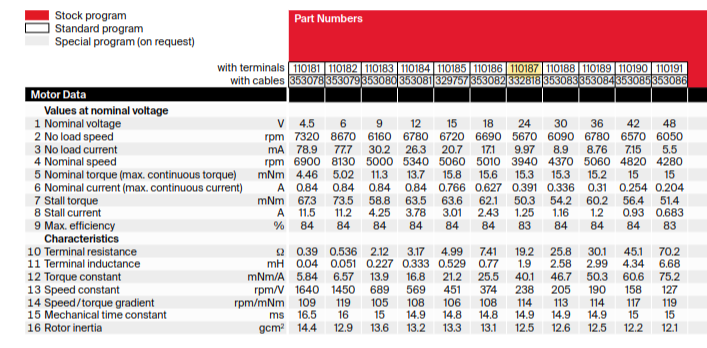
\includegraphics[width=0.9\textwidth]{motorSpec.png}
\end{figure}

I took the parameters from the motor specification table above using part number 110187.
\begin{align*}
    R_M&=19.2\;\Omega \\
    L_M&=1.9\text{mH}=0.0019\text{ H} \\
    K_\tau&=40.1\text{mNm/A}=0.0401\text{ Nm/A}  \\
    J_M&=12.5\text{gcm}^2=0.00000125\text{ kgm}^2 \\
    K_B&=238\text{rpm/V}=0.04\text{ Vs/rad} \\
    N&=33.3 \\
    J_L&=0.018522\text{ kgm}^2 \\
    K_S&=0.8\text{ V/rad}
\end{align*}

I derived N by using the logic that the gear ratio measured in radii is equal to the gear ratio measured in circumferences and if the teeth on both gears are the same size then you could measure the circumference in number of teeth and take the ratio of numbers of teeth.
The load shaft gear has 120 teeth and the motor shaft gear has 36, making the ratio between them 3.33.
The ratio from the motor to the motor shaft gear through the gear head is 10, making the total gear ratio 33.3.
I got the gear head ratio from the spec sheet below:

\begin{figure}[H]
    \centering
    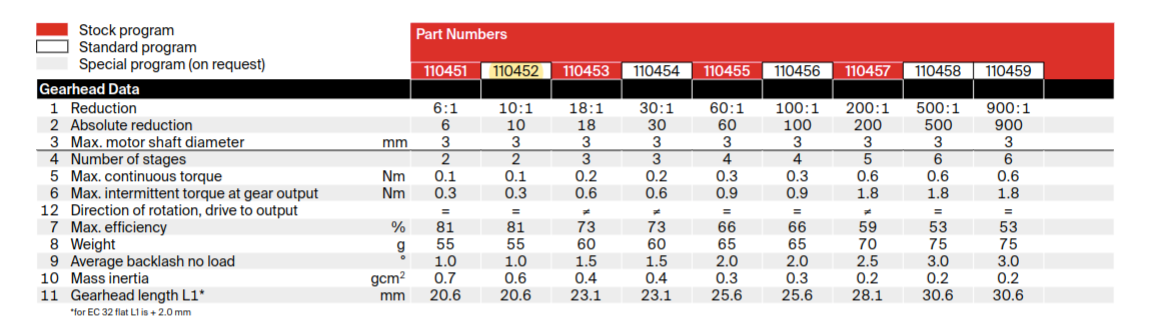
\includegraphics[width=\textwidth]{gearHeadSpec.png}
\end{figure}

I estimated $J_L$, using standard inertia formulas for a rod rotating about one end and a satellite (for the weight) and added them together.
\\
Equation for rod:
$J_{\text{arm}} = \frac{1}{3} m_{\text{arm}} L^2$
\\
Equation for weight:
$J_{\text{weight}} = m_{\text{weight}} L^2$
\\
\\
I got the mass of the arm and weight using their measurements and the average density for aluminum and brass.
\begin{itemize}
    \item Arm Dimensions: \( L = 30 \) cm, \( h = 0.7 \) cm, \( w = 1.1 \) cm
    \item Volume:
    \begin{equation}
        V_{\text{arm}} = L \times h \times w = 30 \times 0.7 \times 1.1 = 23.1 \text{ cm}^3
    \end{equation}
    \item Density of aluminum: \( \rho_{\text{Al}} \approx 2.7 \) g/cm³
    \item Mass of the arm:
    \begin{equation}
        m_{\text{arm}} = V_{\text{arm}} \times \rho_{\text{Al}} = 23.1 \times 2.7 = 62.37 \text{ g} = 0.0624 \text{ kg}
    \end{equation}
\end{itemize}

\begin{itemize}
    \item Weight Dimensions: \( 3.2 \times 2.0 \times 3.4 \) cm
    \item Volume:
    \begin{equation}
        V_{\text{brass}} = 3.2 \times 2.0 \times 3.4 = 21.76 \text{ cm}^3
    \end{equation}
    \item Density of brass: \( \rho_{\text{brass}} \approx 8.5 \) g/cm³
    \item Mass of the brass weight:
    \begin{equation}
        m_{\text{brass}} = V_{\text{brass}} \times \rho_{\text{brass}} = 21.76 \times 8.5 = 184.96 \text{ g} = 0.185 \text{ kg}
    \end{equation}
\end{itemize}

Then I used those numbers (including length of arm for L) to calculate the moments of inertia and combine them.

\begin{equation}
    J_{\text{arm}} = \frac{1}{3} m_{\text{arm}} L^2
\end{equation}

\begin{equation}
    J_{\text{arm}} = \frac{1}{3} (0.0624) (0.30)^2 = 0.001872 \text{ kg}\text{m}^2
\end{equation}

\begin{equation}
    J_{\text{weight}} = m_{\text{weight}} L^2
\end{equation}

\begin{equation}
    J_{\text{weight}} = (0.185) (0.30)^2 = 0.01665 \text{ kg}\text{m}^2
\end{equation}

\begin{equation}
    J_L = J_{\text{arm}} + J_{\text{brass}}
\end{equation}

\begin{equation}
    J_L = 0.001872 + 0.01665 = 0.018522 \text{ kg}\text{m}^2
\end{equation}

\begin{figure}[H]
    \centering
    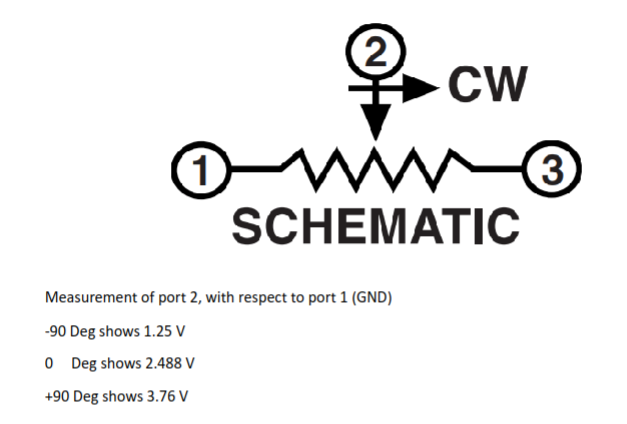
\includegraphics[width=0.8\textwidth]{potentiometerSpec.png}
\end{figure}

To derive $K_S$ I used the readings/schematic above.
I took the total voltage difference over the total angle difference (converted to radians).
\begin{align}
    K_S&=(3.76V-1.25V)/(\frac{\pi}{2}\text{rad}+\frac{\pi}{2}\text{rad}) \\
    K_S&=0.8\text{ V/rad}
\end{align}

The transfer function that relates $V_P$ to $\Theta_L$ is:
\begin{equation}
    \frac{-1}{\frac{1}{NK_{\tau}}J_{eq}L_Ms^3 + \frac{1}{NK_{\tau}}J_{eq}R_Ms^2+NK_Bs}
\end{equation} 

I derived $J_{eq}$ using:

\begin{align*}
    J_{eq} &= J_L + N^2J_M \\
    J_{eq} &= 0.01988325kgm^2
\end{align*}

Plugging in the parameter values:
\begin{equation}
    \frac{-1}{0.000028291\;V\cdot sec^3 \;s^3 + 0.285890679\;V\cdot sec^2\;s^2+1.332\;\frac{V\cdot sec}{rad}\;s}
\end{equation} 

\section*{2.}

\textit{
    "[20pts] Simulate the system relating power amp voltage $V_P$ to sensor voltage $V_S$ using a single
    transfer function block from the Continuous library in Simulink. I suggest you compute
    polynomial coefficients in a separate m-file (as in the intro\_sims.m example), so the simulink
    system can be built using simple variable names from the workspace. Use a sinusoidal power
    amp input voltage (1V peak, 1Hz), and plot the corresponding input and output signals, with
    appropriate units. Does the output follow the input closely?"
}

I set up the variables for the transfer function as suggested in a matlab file as shown below.

\begin{lstlisting}[style=matlabstyle]
coeff3=0.000028291; % [Vs^3]
coeff2=0.285890679; % [Vs^2]
coeff1=1.332; % [Vs/rad]
num = [-1];
den = [coeff3, coeff2, coeff1, 0];
format longG;
poles = roots(den);
disp(poles);

plot(out.inData.time, out.inData.Data, 'b-', ...
     out.outData.time, out.outData.Data, 'r--');

xlabel('Time (s)');
ylabel('Voltage (V)');
legend('Input Vp', 'Sensor Voltage Vs');
title('Open Loop Input vs. Output Voltage');
grid on;
\end{lstlisting}

I then created my model in Simulink using num and den from the m file for the transfer function, a 1V-1Hz sine wave input, and a couple 'To Workspace' blocks so I could plot the input/output.

\begin{figure}[H]
    \centering
    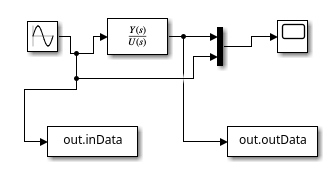
\includegraphics[width=0.8\textwidth]{simulinkOpenModel.png}
\end{figure}

Then I ran the simulation and plotted the results as you can see below:

\begin{figure}[H]
    \centering
    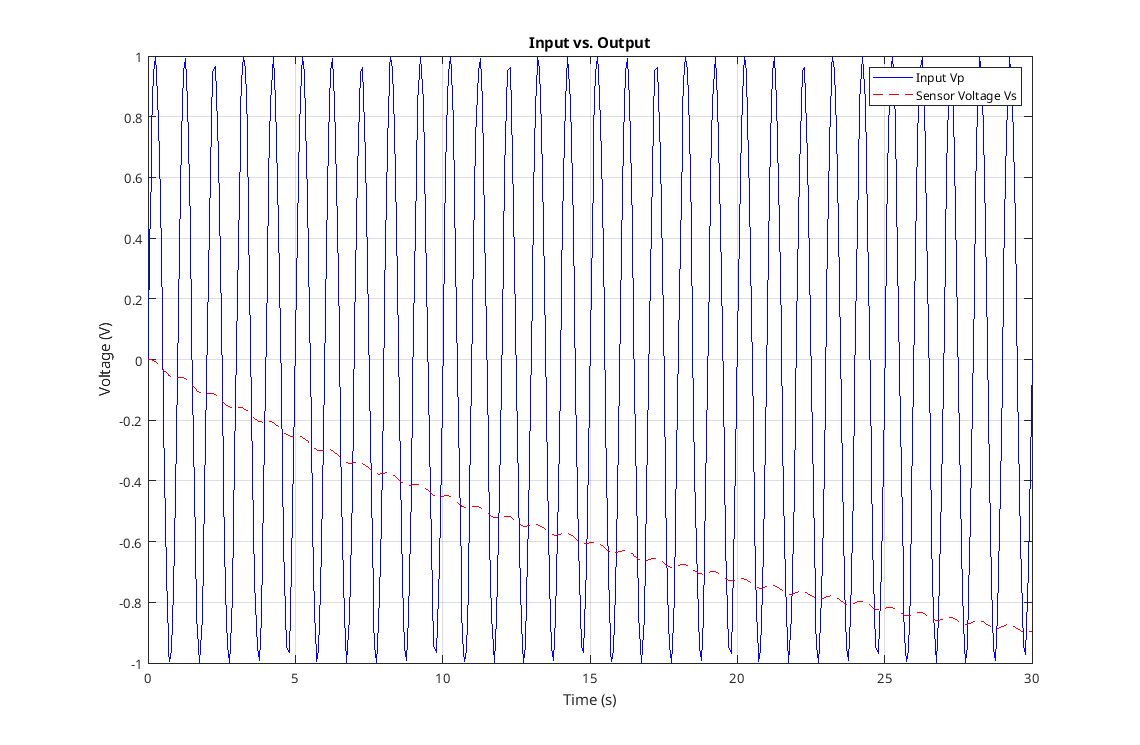
\includegraphics[width=\textwidth]{openPlot.png}
\end{figure}

The output follows the input in that they are both constant, steady sine waves.
However, the magnitude and phase is shifted, the magnitude is attenuated, the output is also shifted down so that the whole signal is negative instead of oscillating between -1 and 1 like thee input.

\section*{3.}

\textit{
    "[10pts] Derive the closed loop transfer function between reference angle
    $\Theta_R$ and load shaft angle $\Theta_L$ when the controller has a 
    proportional-plus-derivative (PD) control law, i.e.
    $V_P = G_P(\Theta_R - \Theta_L) + G_D\frac{d}{dt}(\Theta_R - \Theta_L).$
    Determine the DC gain of the closed loop system."
}

I derived the closed loop transfer function using the closed loop relationship

\[
\frac{\Theta_L}{\Theta_R}=\frac{PC}{1+PC}
\]

Where P is the plant and C is the controller.
I will use the same B/A transfer function for the plant and the proportional and derivative gains for the controller.

\begin{align*}
    P &= \frac{B}{A} \\
    C &= G_P+G_D\frac{d}{dt} \\
    \frac{\Theta_L}{\Theta_R}&=\frac{P(G_P+G_D\frac{d}{dt})}{1+P(G_P+G_D\frac{d}{dt})}
\end{align*}

The DC gain of the closed loop system can be derived by converting the transfer function to the LaPlace domain and getting the value as s goes to 0.

\[
\frac{\Theta_L}{\Theta_R}=\frac{P(s)(G_P+G_Ds)}{1+P(s)(G_P+G_Ds)}
\]

This can be rewritten as:

\[
\frac{\Theta_L}{\Theta_R}=\frac{(G_P+G_Ds)}{\frac{1}{P(s)}+(G_P+G_Ds)}
\]

$\frac{1}{P(s)}$ goes to 0 since the plant is -1 over a few powers of s, the reciprocal of that is just negative a few powers of s which all go to 0.
$G_Ds$ also goes to 0 so you are left with $\frac{G_P}{G_P}$ which is 1.

\section*{4.}

\textit{
    "[20pts] Construct a Simulink model of the control system including both proportional and
    derivative control. DO NOT create one block that represents the closed loop transfer function
    derived in Part 3. Instead, create a second block for the control law itself and then connect it in a
    unity-feedback control system with the Plant block from part 2. Label this block diagram with
    signal names and units"
}
\\
\\
I constructed the closed loop model using the same plant from the open loop, the PID Controller Block which I just set to PD and set the gains to -10 and -0.1 and left the filter coefficient at 100 because I don't really understand it but I believe it is intended to stabilize the signal at high frequencies, and then I put in a step source instead of the sine wave source.

\begin{figure}[H]
    \centering
    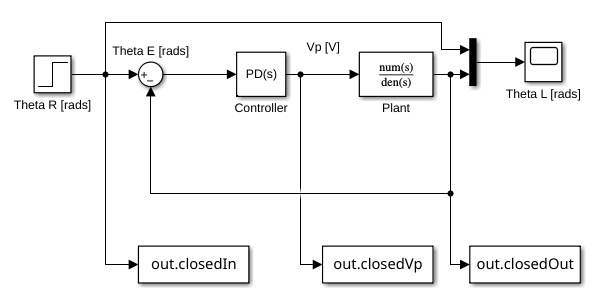
\includegraphics[width=\textwidth]{closedModel.png}
\end{figure}

\section*{5.}

\textit{
    "[10pts] Plot the simulated step response (0.4 radian amplitude) of this closed loop control
    system using a proportional gain of 10 V/rad and a derivative gain of 0.1 V/rad/s . Compare the
    steady state tracking behavior to that predicted by the DC gain calculated in part 3."
}
\\
\\
\begin{figure}[H]
    \centering
    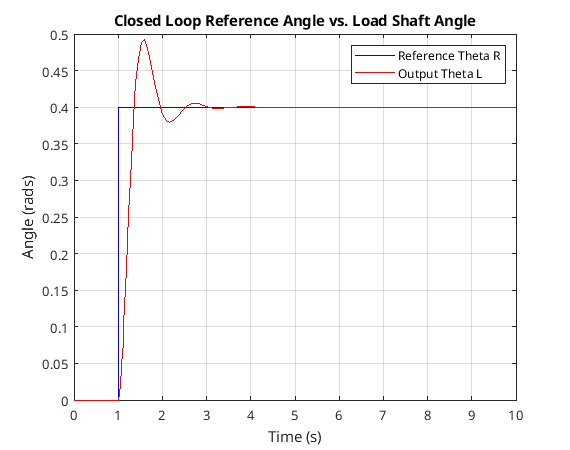
\includegraphics[width=0.8\textwidth]{closedLoopStepPlot.png}
\end{figure}

The steady state tracking behavior is right on, after the natural response oscillation settles the output settles to exactly the same value as the input.

\section*{6.}

\textit{
    "[20pts] Repeat part 5, but use sinusoid reference signals at 0.4 rad amplitude, with frequencies
    of 0.2 Hz and 2 Hz. Comment on the relative tracking ability of the system at these two
    frequencies."
}
\\
\\
\begin{figure}[H]
    \centering
    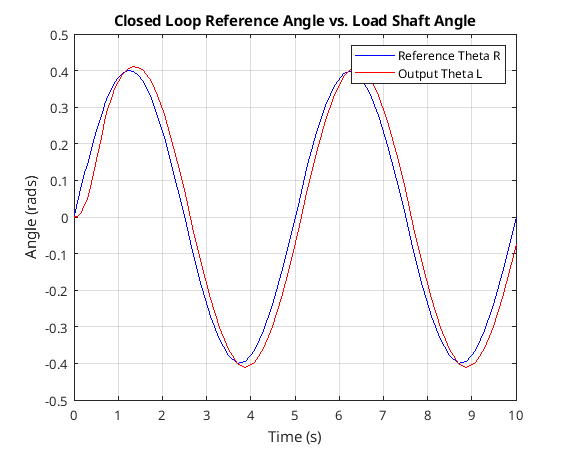
\includegraphics[width=0.8\textwidth]{closedSinePoint2Hz.png}
\end{figure}

\begin{figure}[H]
    \centering
    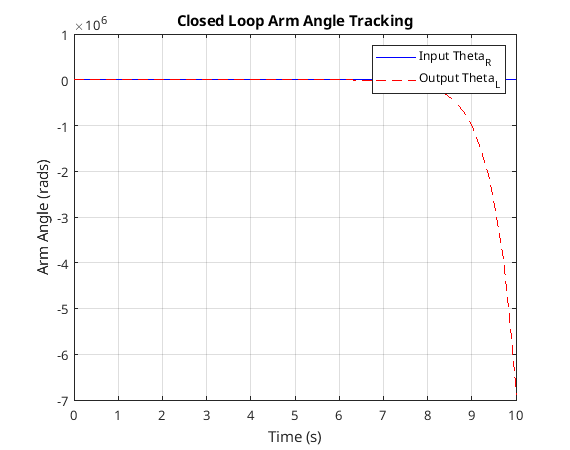
\includegraphics[width=0.8\textwidth]{closedSine2Hz.png}
\end{figure}

At 0.2 Hz the output tracks the input pretty closely though there is a bit of a phase shift delay.
At the higher 2 Hz frequency you can see much more of a phase shift and an attenuation of the magnitude.
The s in the denominator of the transfer function create integration-like behavior and when the frequency is lower those s terms don't have much effect but as it goes higher the s terms dominate and decrease the gain and introduce more of a phase shift.

\bigskip

Below is from an earlier version of this document where I had not included the gearhead ratio in the N calculation and I was using positive gains in my closed loop PD block so the calculations were slightly off and the closed loop gains were causing the system to go unstable so I had a bunch of exploding outputs.
I'm leaving the notes here because they are interesting and informative and I fully derive the closed loop transfer function and its poles which might be useful information later.

\bigskip

Okay, I think I figured out the issue.
I wrote out the closed loop transfer function so I could derive those roots and see what the behavior should look like.

Starting from the transfer function I derived above:
\[
\frac{\theta_L(s)}{\theta_R(s)} = \frac{P(s) \cdot (G_P + G_D s)}{1 + P(s) \cdot (G_P + G_D s)}
\]

Substitute \(P(s)\) with the plant's transfer function:
\[
P(s) = \frac{-1}{0.000266135 s^3 + 2.6893656 s^2 + 0.132 s}
\]

Therefore, the closed-loop transfer function becomes:
\[
\frac{\theta_L(s)}{\theta_R(s)} = \frac{\left(\frac{-1}{0.000266135 s^3 + 2.6893656 s^2 + 0.132 s}\right) \cdot (G_P + G_D s)}{1 + \left(\frac{-1}{0.000266135 s^3 + 2.6893656 s^2 + 0.132 s}\right) \cdot (G_P + G_D s)}
\]

Simplify the expression:
\[
\frac{\theta_L(s)}{\theta_R(s)} = \frac{-(G_P + G_D s)}{0.000266135 s^3 + 2.6893656 s^2 + 0.132 s - G_P - G_D s}
\]

Combine like terms in the denominator:
\[
\frac{\theta_L(s)}{\theta_R(s)} = \frac{-(G_P + G_D s)}{0.000266135 s^3 + 2.6893656 s^2 + (0.132 - G_D) s - G_P}
\]

The final closed-loop transfer function is:
\[
\frac{\theta_L(s)}{\theta_R(s)} = \frac{-G_D s - G_P}{0.000266135 s^3 + 2.6893656 s^2 + (0.132 - G_D) s - G_P}
\]

I used the built-in roots function to get the roots of this transfer function in Matlab.

\begin{lstlisting}[style=matlabstyle]
Gp = 10;
Gd = 0.1;
numCL = [-Gd -Gp];
denCL = [0.000266135, 2.6893656, 0.132 - Gd, -Gp];
disp(roots(denCL));
\end{lstlisting}

Results:
-10105.2561121366
-1.9344463849097
1.92217969120724

Aha! A positive root. Not good.

I changed the gains to be negative and look:

\begin{figure}[H]
    \centering
    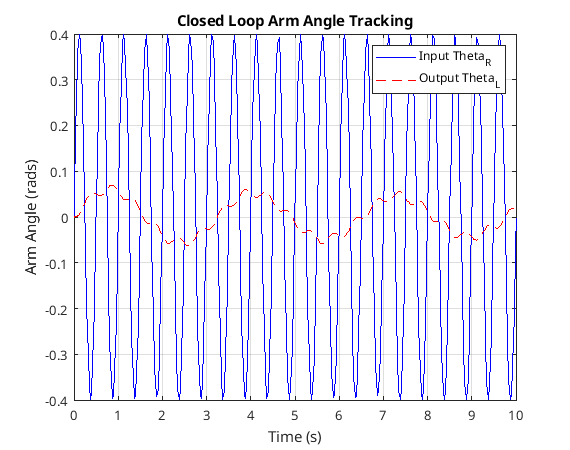
\includegraphics[width=0.8\textwidth]{negativeGain.png}
\end{figure}

That's the 2Hz sine with -10 proportional gain and -0.1 derivative gain.
Not exactly tracking but stable.
I suspect this was either a trick question type situation or my calculations missed a sign somewhere tragically.
More investigation required.

\end{document}